\chapter{Análise Bibliográfica sobre Criptografia no Universo da Computação Quântica, por André Larrosa Chimpliganond}

\section{Planejamento do estudo}
Como se transmitir informações de modo que esta só possa ser acessada pela pessoa certa? Responder essa pergunta e elaborar métodos para por a solução em prática é área de estudo da criptografia. Utilizando de alta complexidade matemática, técnicas de criptografia codificam informações de modo que só possam ser decodificadas por quem possuir a chave. Mas como o advento e evolução da computação quântica afeta a maneira como criptografamos os dados?

Partindo dessa pergunta, podemos explorar outras que irão nortear o trabalho:
\begin{itemize}
    \item Quais conceitos relacionados à esse embate entre a criptografia e computação quântica?
    \item Quais autores, instituições e nações estão à frente desse tema?
    \item Como esse conteúdo tem se desenvolvido ao longo do tempo?
\end{itemize}



% nao sei se vou colocar
\subsection{O que já existe de pesquisa bibliométrica sobre esse tema?}

\cite{gore_classifying_2016} fizeram uma pesquisa que visava aprofundar a questão da simulação multiagente em relação à computação experimental.

A pesquisa é base para um posterior aprofundamento no campo da Cientometria, como fez \cite{chavalarias_whats_2017}.
% 

\subsection{Ferramentas}
Será utilizada a interface web para o pacote Bibliometrix (Biblioshiny). O pacote Bibliometrix é uma ferramenta R que fornece um conjunto de ferramentas para a investigação quantitativa em cientometria e bibliometria.


% nao sei se vou colocar
\subsection{Limitações} O exercício relatado foi feito em uma semana, envolvendo entre 5 a 10 horas de trabalho de cada autor.

Outros aspectos a reforçar:
\begin{itemize}
   
\item Deve-se fazer buscas na base de dados WoS ou SCOPUS;
\item é obrigatório declarar um conjunto de perguntas de pesquisa.
\item é preciso declarar o objetivo da pesquisa, que no caso da aqui relatada foi exercitar inicialmente, e relatar, o uso da técnica de análise bibliométrica, para fins didáticos.
\end{itemize}
%

\section{Coleta de dados}%label

A coleta de dados feita usando o Web Of Science  no dia 09 de fevereiro de 2022, acessado por meio do Portal de Periódicos da CAPES.

Foram feitas buscas nas coleções \textbf{Science Citation Index Expanded (SCI-EXPANDED)--1945-presente}, \textbf{Conference Proceedings Citation Index – Science (CPCI-S)--1990-presente} e \textbf{Emerging Sources Citation Index (ESCI)--2017-presente}. 

Foi usada a seguinte \query\  de busca

\lstinputlisting[numbers=left,basicstyle=\normalsize\ttfamily,caption={\query\  de busca sobre criptografia quântica.}]%label
%{experiments/andrelarrosacrypt/AnaliseBibliometrica/CriptografiaQuantica/query.txt}
%nao ta achando a query

\subsection{Explicação para os termos de busca usados}%label

Foram elaboradas duas cláusulas de busca unidas por \textit{and}. A primeira foca nos elementos relacionados ao universo quântico, enquanto a segunda faz referência à criptografia.


Os 10522 registros obtidos encontram-se no github do projeto, em \url{https://github.com/jhcf/Comput-Experim-20212/experiments/andrelarrosacrypt/AnaliseBibliometrica/CriptografiaQuantica/rec_1.txt} e \url{https://github.com/jhcf/Comput-Experim-20212/experiments/andrelarrosacrypt/AnaliseBibliometrica/CriptografiaQuantica/rec_2.txt}. 
% enviar arquivo completo direto no github

Foram exportadas todas as informações disponíveis na Web Of Science de cada documento.

\section{Análise dos dados}

\subsection{Filtragem de registros}


Após carregar o dataset na plataforma biblioshiny, foi feita uma filtragem dos documentos com o intuito de selecionar apenas os artigos publicados em revistas científicas (\textit{ARTICLE}). Após a filtragem, sobraram 7131 documentos. Esse novo dataset será nomeado CriptografiaQuanticaArtigos ou CQA@andrelarrosacrypt.

\subsection{Informações principais do \dataset\   CQA@andrelarrosacrypt}
\begin{description}
    \item[Período]	1988 - 2022
    \item[Fontes]	675
    \item[Documentos]	7131
    \item[Média de tempo de publicação]	8.31
    \item[Média de citações por documento]	33.05
    \item[Média de citações por ano por documento]	2.75
    \item[Referências]	83981
    \item[Palavras-chave (Keywords Plus (ID))]   3187
    \item[Palavras-chave (Author's Keywords (DE))] 8201
    \item[Autores]   10925
    \item[Aparições de autores]	28034
    \item[Autores de documentos de autoria única]	436
    \item[Autores de documentos de autoria múltipla]	10489
    \item[Documentos de autoria única]	706
    \item[Média de documentos por autor]	0.653
    \item[Média de autores por documento]	1.53
    \item[Média de co-autores por documento]	3.93
    \item[Index de colaboração]        1.63
\end{description}


\subsection{Evolução da Produção Científica}

\begin{figure}
    \centering
    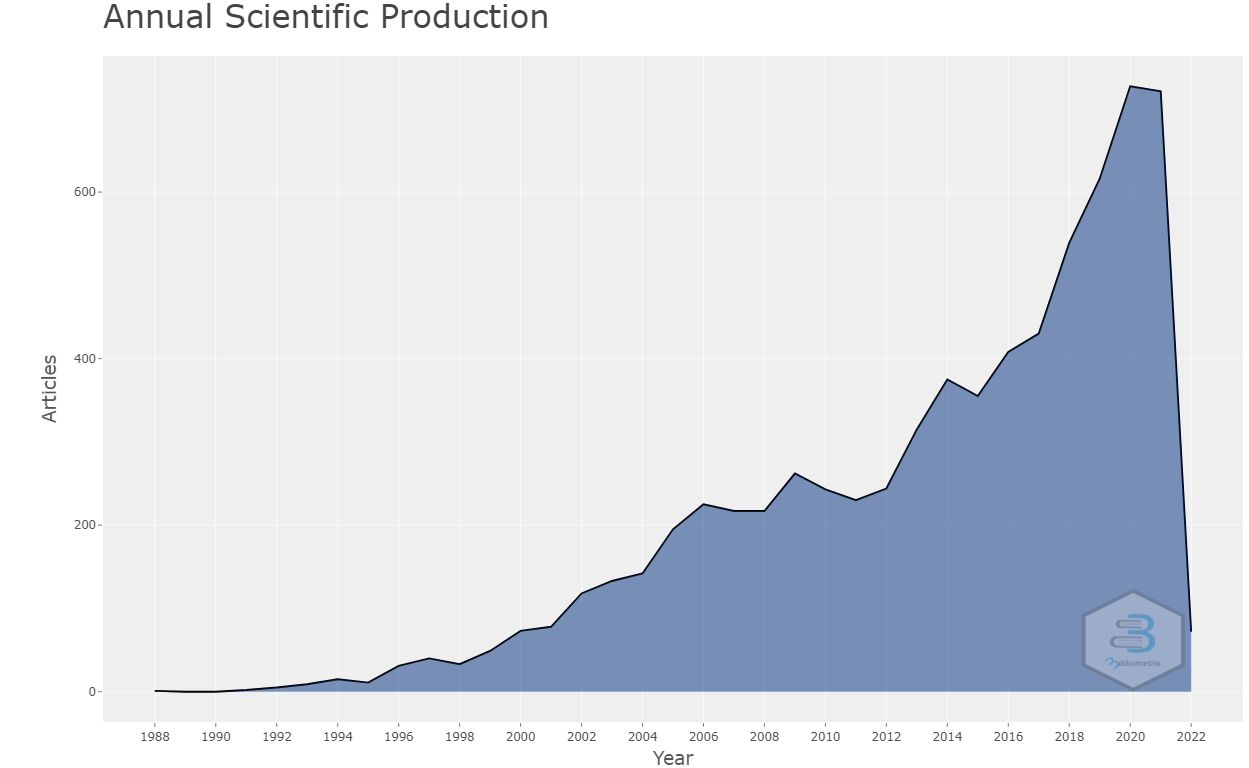
\includegraphics[width=1\textwidth]{experiments/andrelarrosacrypt/AnaliseBibliometrica/CriptografiaQuantica/imagens/CQA@andrelarrosacrypt_ProdAnual.png}
    \caption{Evolução da produção científica no \dataset\ CQA@andrelarrosacrypt.}
    \label{CQA@andrelarrosacrypt_ProdAnual}
\end{figure}

A figura \ref{CQA@andrelarrosacrypt_ProdAnual} representa a evolução da produção de documentos relacionados ao tema do \dataset\ CQA@andrelarrosacrypt, de 1988 até 2022. Como os dados foram coletados no início de 2022, a produção específica desse ano ainda é baixa, mas, como o gráfico segue uma curva aproximadamente exponencial, é de se esperar que acompanhe o nível de 2020 e 2021.



\subsection{Interpretação do Crescimento}
% colocar ref em @, quantum computing timeline

Como destacado em \url{https://www.quthought.com/post/history-of-quantum-computing-a-timeline}, o do desenvolvimento da computação quântica nos anos 1990 é representado na figura como o início do crescimento das pequisas. Na mesma referência, percebemos que nos últimos dez anos empreses como Google e IB, além de instituições como NASA e NSA tem investido nesse assunto. Indicando, não só um interesse econômico, mas uma necessidade governamental.

Se considerarmos os interesses da NSA (Agência de Segurança Nacional dos Estados Unidos), percebemos como esse novo tipo de computação está alterando a meneia como vemos codificação e decodificação de informações. 


\subsection{Evolução das Citações}

\begin{figure}
    \centering
    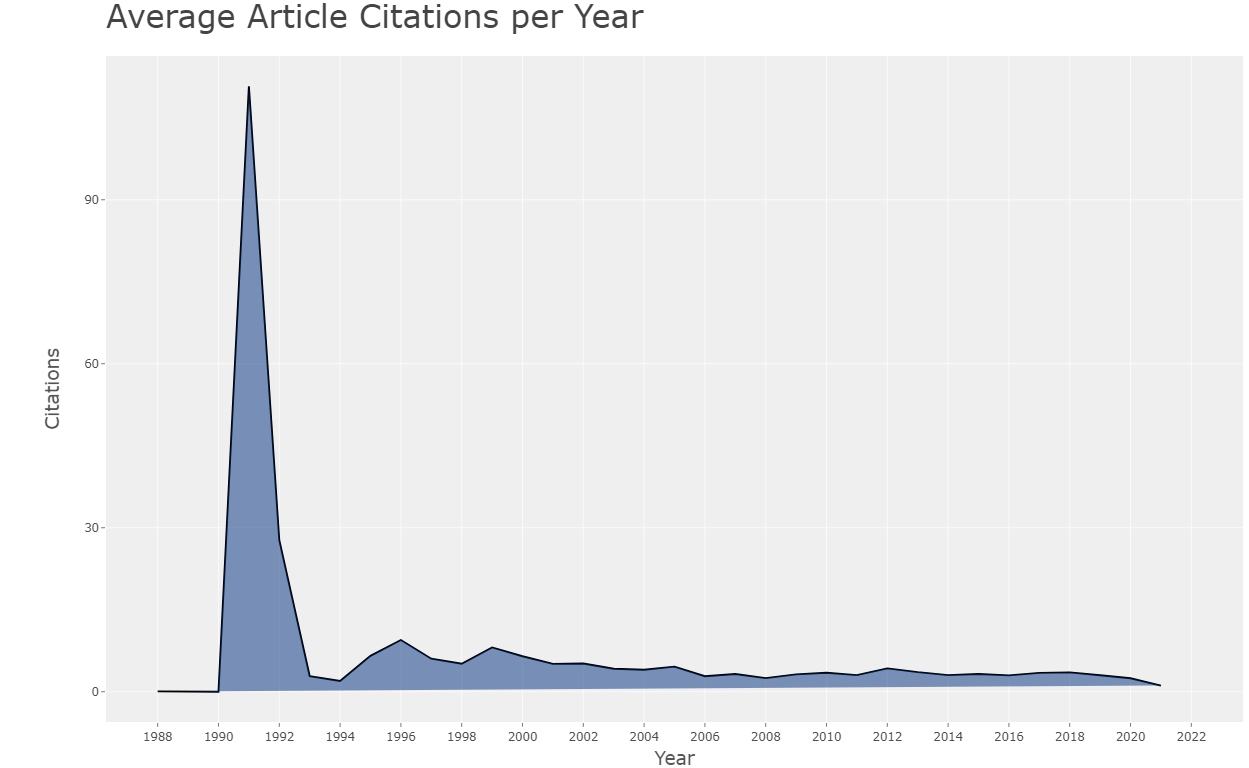
\includegraphics[width=1\textwidth]{experiments/andrelarrosacrypt/AnaliseBibliometrica/CriptografiaQuantica/imagens/CQA@andrelarrosacrypt_CitaAnual.png}
    \caption{Evolução das citações ao \dataset\ CQA@andrelarrosacrypt.}
    \label{CQA@andrelarrosacrypt_CitaAnual}
\end{figure}

% media das citacoes ?????/

Como mostrado na figura \ref{CQA@andrelarrosacrypt_CitaAnual}, com exceção aos anos 1990 e 1991, os documentos apresentam uma média de ???.


\subsection{Interpretação das Citações}

% n de citacoes nao cresce



% artigos mais importantes ???


\subsection{\textit{Three-Field Plots}}

Gráficos do tipo \textit{Three-Field Plots} exibem três campos (autores, documentos, referências, entre outros) e como eles se relacionam (\textit{Three-Field Plots}).

\subsection{\textit{Three-Field Plots} Autores, Referências e Palavras-chave}

\begin{figure}
    \centering
    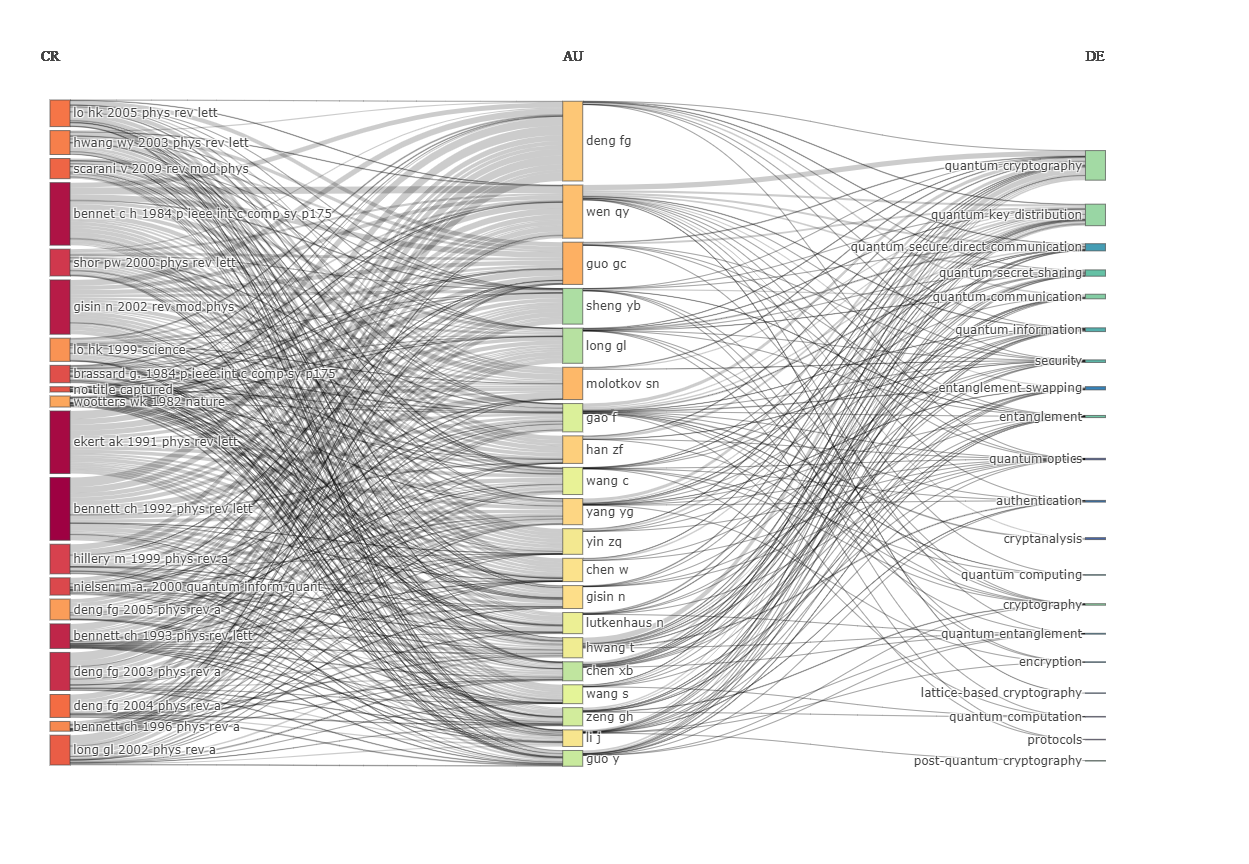
\includegraphics[angle=0,width=1\textwidth]{experiments/andrelarrosacrypt/AnaliseBibliometrica/CriptografiaQuantica/imagens/CQA@andrelarrosacrypt_Aut_Ref_Key.png}
    \caption{\textit{Three-Field Plots} do \dataset\ CQA@andrelarrosacrypt: 20 Autores, 20 Referências e 20 Palavras-Chave mais relevantes.}
    \label{CQA@andrelarrosacrypt_Aut_Ref_Key}
\end{figure}

A figura \ref{CQA@andrelarrosacrypt_Aut_Ref_Key} apresenta o gráfico \textit{Three-Field Plots} do  \dataset\ CQA@andrelarrosacrypt. Os campos de interesse destacados nesse gráfico são autores (centro), referência citadas (esquerda) e palavras-chave (direita) mais importantes.


\subsubsection{Interpretação da figura \ref{CQA@andrelarrosacrypt_Aut_Ref_Key}}

No campo \textit{autores}, percebemos que 19 aparentam ser de origem asiática (mais provavelmente chinesa), o único não asiático provavelmente é russo (molotkov sn). Por outro lado, as referências apresentam maior heterogeneidade, com documentos aparentemente asiáticos, europeus e norte-americanos. Isso nos sugere que pesquisadores de origem chinesa tem migrado para países ocidentais ou tem trabalhado em direta colaboração com pesquisadores europeus e norte-americanos.

Relevante cometar que o autor mais destacado é \textbf{deng fg} e nas referências mais citadas temos três trabalhos de sua autoria \textbf{}{Deng FG, 2003, PHYS REV A} - DOI 10.1103/PhysRevA.68.042317 (protocolo para comunicação quântica segura), \textbf{Deng FG, 2004, PHYS REV A} - DOI 10.1103/PhysRevA.69.052319 (outro protocolo para comunicação quântica segura) e \textbf{Deng FG, 2005, PHYS REV A} - DOI 10.1103/PhysRevA.72.044302 (análise de protocolo de comunicação segura proposto por Zhang, Li, and Man). O que nos mostra a relevância de tal autor e seu aparente foco na área de comunicação segura.

Ao estudarmos as \textit{palavras-chaves} fica claro o focos desses autores no temos de comunicação quântica segura, \textbf{quantum secure direct communication}, \textbf{quantum secret sharing} e \textbf{quantum communication}, e o uso de criptografia quântica, \textbf{quantum cryptography} e \textbf{quantum key distribution}, para tal fim.


\subsection{\textit{Three-Field Plots} Autores, Afiliações e Países}

\begin{figure}
    \centering
    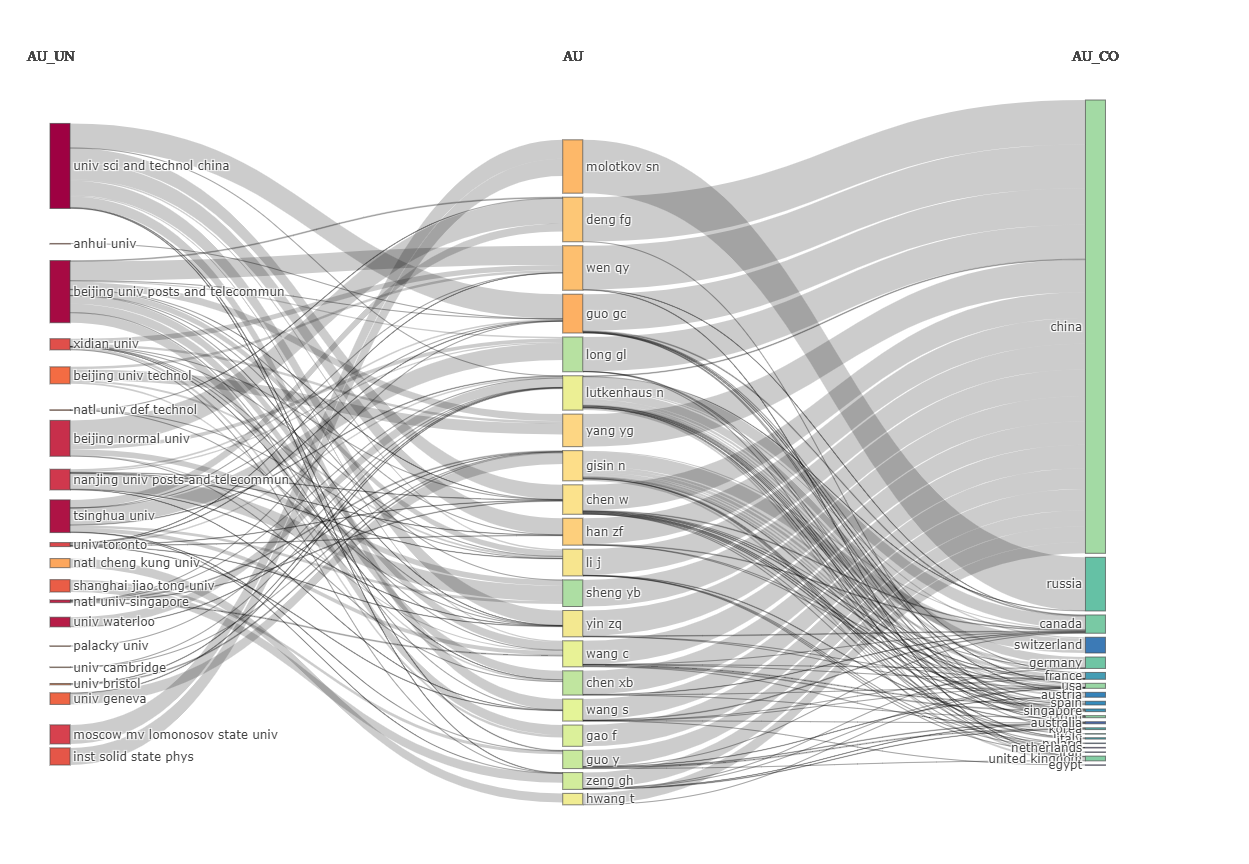
\includegraphics[angle=0,width=1\textwidth]{experiments/andrelarrosacrypt/AnaliseBibliometrica/CriptografiaQuantica/imagens/CQA@andrelarrosacrypt_Aut_Aff_Coun.png}
    \caption{\textit{Three-Field Plots} do \dataset\ CQA@andrelarrosacrypt: 20 Autores, 20 Instituições e 20 Países mais relevantes.}
    \label{CQA@andrelarrosacrypt_Aut_Aff_Coun}
\end{figure}

\subsubsection{Interpretação da figura \ref{CQA@andrelarrosacrypt_Aut_Aff_Coun}}

O gráfico da figura \ref{CQA@andrelarrosacrypt_Aut_Aff_Coun} confirma as suspeitas em relação à origem chinesas da maioria dos autores. Mesmo com a prevalência da China, temos a Rússia, Canada, Suíça, Alemanha, França e Estados Unidos com significativa influência.

Com relação às instituições afiliadas, notamos um predomínio das universidades chinesas, o que pode indicar que esses pesquisadores chineses estão trabalhando na China e não em universidades estrangeirais como havia sido sugerido. Observando o campo dos países, percebemos que muitos dos pesquisadores chineses tem afiliações com outros países. Isso indica que a segunda teoria apontada anteriormente, colaboração com pesquisadores ocidentais, parece ser verdade.

\section{Estrutura Conceitual}

\begin{figure}
    \centering
    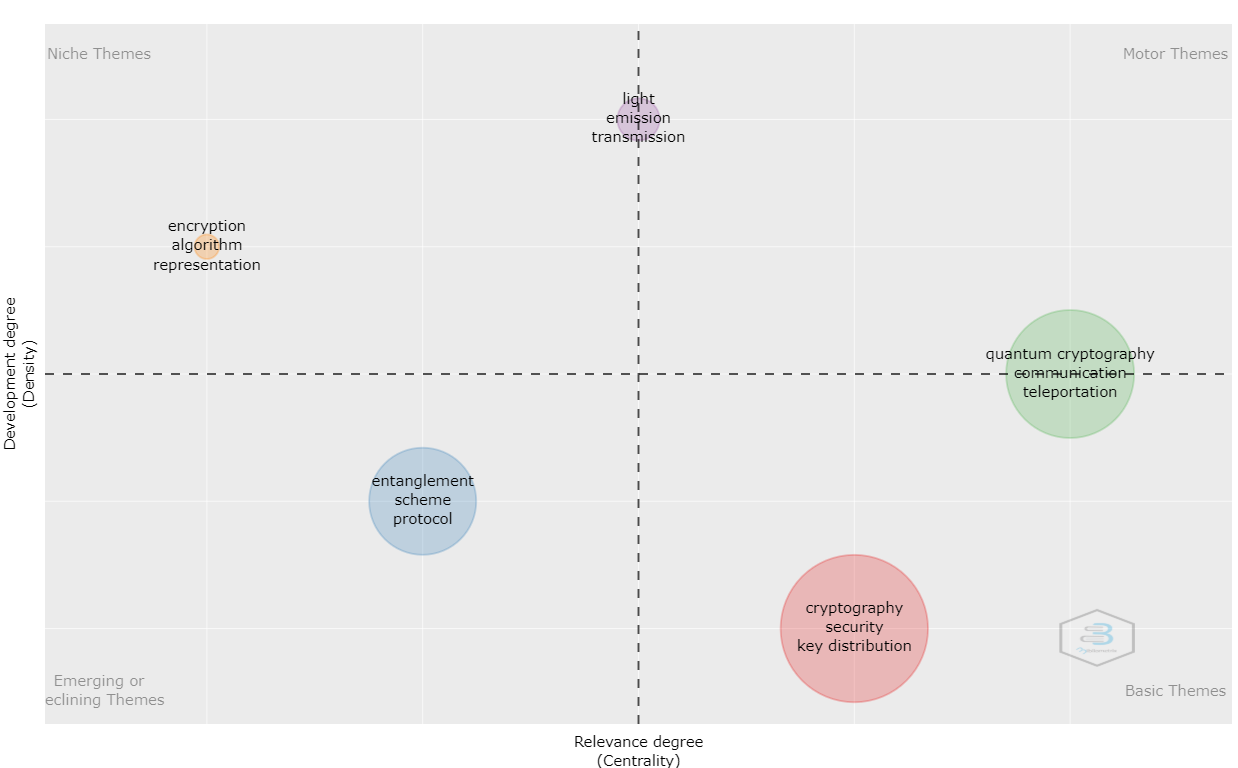
\includegraphics[angle=0,width=1\textwidth]{experiments/andrelarrosacrypt/AnaliseBibliometrica/CriptografiaQuantica/imagens/CQA@andrelarrosacrypt_MapaTematico.png}
    \caption{Mapa temático do \dataset\ CQA@andrelarrosacrypt.}
    \label{CQA@andrelarrosacrypt_MapaTematico}
\end{figure}

Fazendo um estudo da figura \ref{CQA@andrelarrosacrypt_MapaTematico} identificamos cinco aglomerados de conceitos que definem as principais áreas de estudo. Termos como \textbf{cryptograpy}, \textbf{quantum cryptograpy}, \textbf{entanglement}, \textbf{algorithm}  são esperados considerando o tema do nosso estudo. O que mais interessa são as expressões que, a priori, não parecem condizer com a pesquisa, essas que vamos focar.

Primeiro, temos em azul duas palavras que necessitam de explicação, \textbf{scheme} e \textbf{protocol}. Ambas fazem referência à comunicação segura e suas regras no mundo quântico. Passando para o aglomerado vermelho, encontramos \textbf{key distribution} está relacionado à um problema em criptografia que envolve a distribuição de chaves de acesso às partes interessadas, o que faz sentido considerando as demais expressões nesse mesmo aglomerado. Com relação ao agregado verde, temos \textbf{teleportation}. Ela se refere à teletransportação quântica, um método de se transferir informação quântica. Por fim, temos o bloco roxo, \textbf{light}, \textbf{emission} e \textbf{transmission}, todos apontam para as ótica quântica que estuda, dentre outras coisas, o uso de fótons de luz para transportar/processar informação.

\section{Estrutura Intelectual}

\begin{figure}
    \centering
    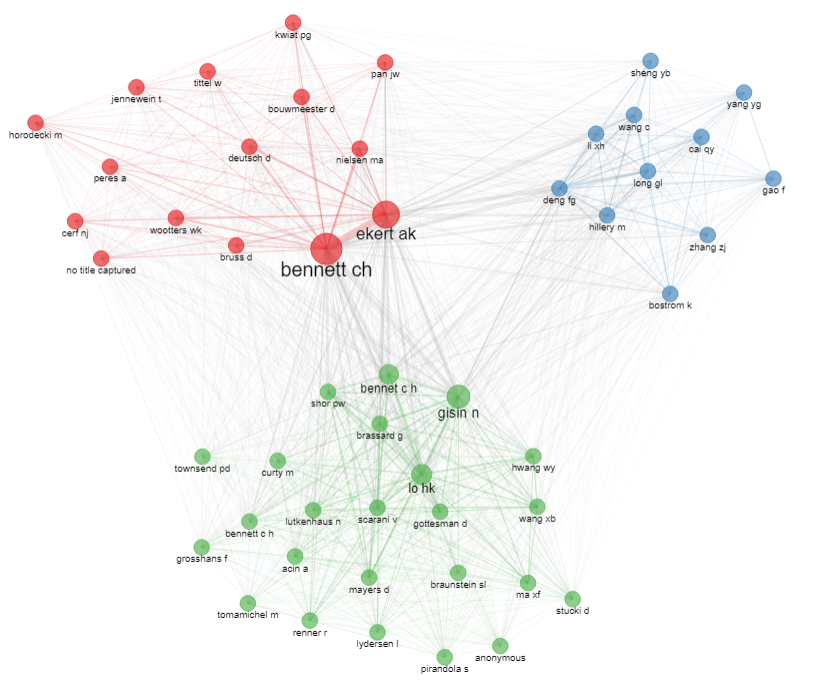
\includegraphics[angle=0,width=1\textwidth]{experiments/andrelarrosacrypt/AnaliseBibliometrica/CriptografiaQuantica/imagens/CQA@andrelarrosacrypt_CoCit.png}
    \caption{Rede de co-citação do \dataset\ CQA@andrelarrosacrypt.}
    \label{CQA@andrelarrosacrypt_CoCit}
\end{figure}

Com relação à estrutura intelectual visível na figura \ref{CQA@andrelarrosacrypt_CoCit}, temos três principais grupos. Em vermelho, encontramos o que parecem ser autores ocidentais, em azul, autores chineses e em verde autores ocidentais e chineses.
% o que mais ??

\section{Estrutura Social}

\begin{figure}
    \centering
    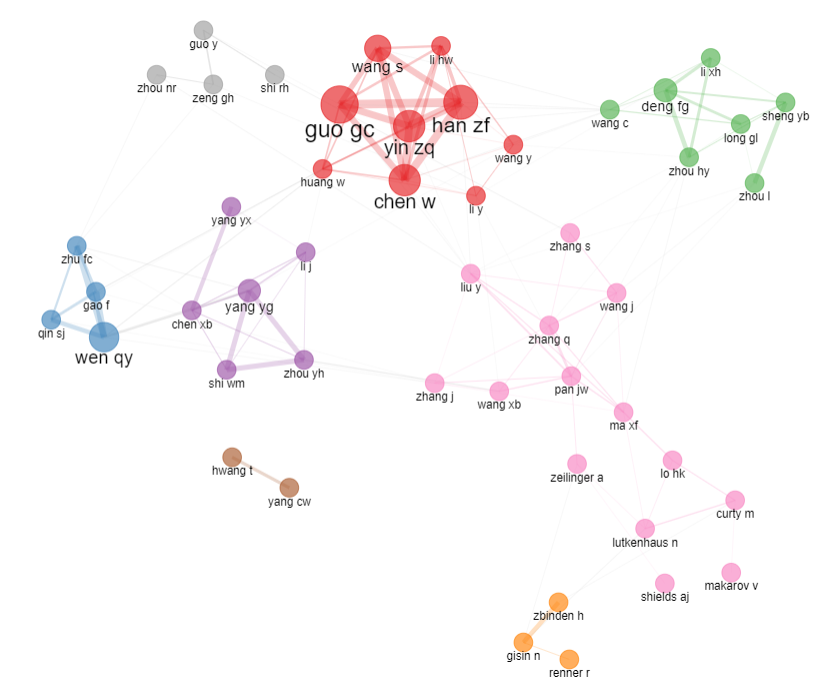
\includegraphics[angle=0,width=1\textwidth]{experiments/andrelarrosacrypt/AnaliseBibliometrica/CriptografiaQuantica/imagens/CQA@andrelarrosacrypt_Colab.png}
    \caption{Rede de colaboração do \dataset\ CQA@andrelarrosacrypt.}
    \label{CQA@andrelarrosacrypt_Colab}
\end{figure}

Na figura \ref{CQA@andrelarrosacrypt_Colab} vemos as colaborações entre autores. Os grupos parecem ser divididos em instituições, com exceção dos autores em rosa que são de instituições distintas. O grupo rosa parece correlacionar com as colaborações entre pesquisadores chineses e ocidentais descrita anteriormente.

\begin{figure}
    \centering
    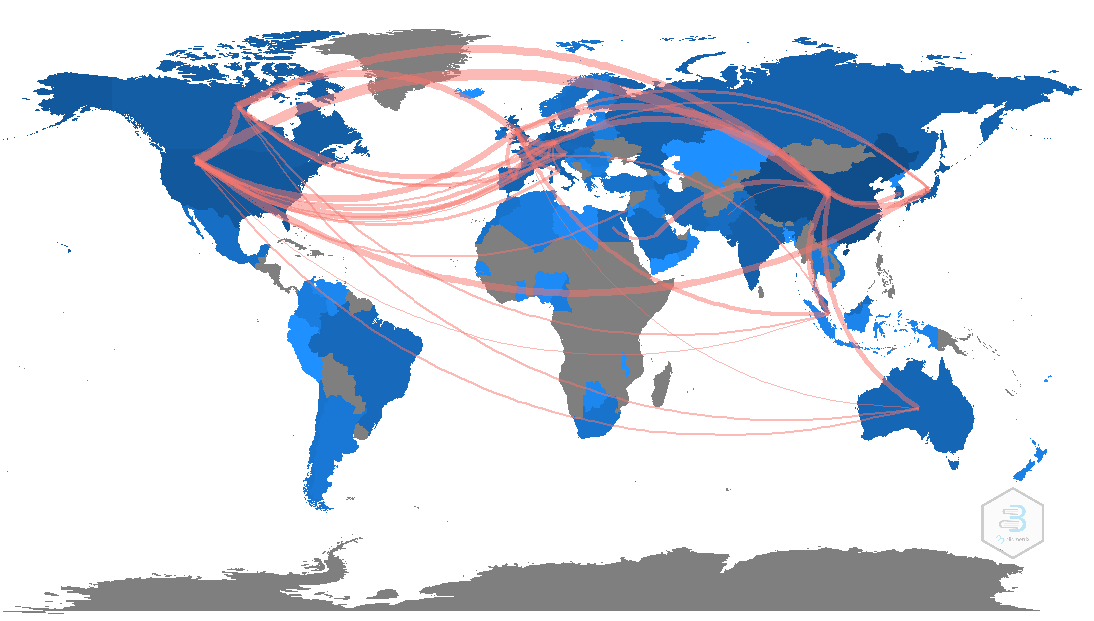
\includegraphics[angle=0,width=1\textwidth]{experiments/andrelarrosacrypt/AnaliseBibliometrica/CriptografiaQuantica/imagens/CQA@andrelarrosacrypt_ColabMap.png}
    \caption{Mapa de colaboração do \dataset\ CQA@andrelarrosacrypt.}
    \label{CQA@andrelarrosacrypt_ColabMap}
\end{figure}

Complementando as informações anteriores, na figura \ref{CQA@andrelarrosacrypt_ColabMap} evidencia as colaborações entre:

\begin{itemize}
    \item China - Estados Unidos
    \item China - Canada
    \item China - Alemanha
    \item China - Reino Unido
    \item Estados Unidos - Canada
    \item Estados Unidos - Reino Unido
\end{itemize}

Com enfase na relação Estados Unidos - China. Esses dados estão de acordo com o cenário geral de pesquisa científica, com norte-americanos e chineses dominando as áreas de conhecimento.